% SELECT COUNT(*) FROM Wallet WHERE inferred=0; (before clustering)
\newcommand{\startingNumberAllWallets}{10477}

% SELECT COUNT(*) FROM Wallet WHERE Status != -1 and inferred=0; (before
% clustering)
\newcommand{\startingNumberWalletsNotService}{6603}

% SELECT COUNT(*) FROM Wallet WHERE Status = 1; (before clustering)
\newcommand{\startingNumberWalletsAtLeastOneTransaction}{1741}

% SELECT COUNT(*) FROM Wallet WHERE 1; (after clustering)
\newcommand{\clusteringNumberAllWallets}{16910}

% SELECT COUNT(*) FROM Wallet WHERE Status != -1; (after clustering)
\newcommand{\clusteringNumberWalletsNotService}{13036}

% SELECT COUNT(*) FROM Wallet WHERE Status != -1 AND Currency='BTC' and
% inferred=0;
% (before clustering)
\newcommand{\startingBTC}{1953}

% SELECT COUNT(*) FROM Wallet WHERE Status != -1 AND Currency='DOGE' and
% inferred=0;
% (before clustering)
\newcommand{\startingDOGE}{654}

% SELECT COUNT(*) FROM Wallet WHERE Status != -1 AND Currency='LTC' and
% inferred=0;
% (before clustering)
\newcommand{\startingLTC}{813}

% SELECT COUNT(*) FROM Wallet WHERE Status != -1 AND Currency='XMR' and
% inferred=0 ;
\newcommand{\startingXMR}{228}

% SELECT COUNT(*) FROM Wallet WHERE Status != -1 AND Currency='ETH' and
% inferred=0;
\newcommand{\startingETH}{2953}

% SELECT COUNT(*) FROM Account WHERE 1;
\newcommand{\accountNumber}{3444}

% SELECT (x*1.0)/((y-1)*1.0) FROM
% (
%     SELECT COUNT(*) AS x
%     FROM Wallet
%     WHERE Wallet.Status != -1
% ),
% (
%     SELECT COUNT(*) AS y
%     FROM Account
% )
\newcommand{\avarageAccount}{$~$3.786}

%~ SELECT COUNT(*) FROM (SELECT DISTINCT * FROM AccountRelated)
\newcommand{\accountRelated}{275}

%~ SELECT count(*) FROM Account WHERE host = 'twitter.com'
\newcommand{\accountTwitter}{888}

%~ SELECT sum(x, y) FROM SELECT count(*) as x FROM Account WHERE host =
% 'github.com',
\newcommand{\accountGithub}{2215}

%~ SELECT count(*) as y FROM Account WHERE host LIKE 'bitcointalk.org'
\newcommand{\accountBitcointalk}{337}

%~ SELECT count(*) FROM Account WHERE host LIKE 'gitlab.com'
\newcommand{\accountGitlab}{2}

%~ SELECT count(*) FROM Account WHERE host LIKE 'bitbucket.org'
\newcommand{\accountBitbucket}{1}

\newcommand{\facebookRelatedAccounts}{12}
\newcommand{\linkedinRelatedAccount}{30}



\section{Results} \label{results}

After we implemented and tested \texttt{Nduja} we ran it. The first step
(\texttt{data retrieving}) of the algorithm  was performed between
17\textsuperscript{th} and 24\textsuperscript{th} February 2018 and gave us
\startingNumberAllWallets{} addresses, \startingNumberWalletsNotService{}
addresses that probably are not services, but we were able to attest that only
\startingNumberWalletsAtLeastOneTransaction{} of them had at least one
transaction. We found out \startingBTC{} Bitcoin addresses, \startingLTC{}
Litecoin addresses, \startingDOGE{} Dogecoin addresses, \startingETH{} Ethereum
addresses and finally \startingXMR{} Monero addresses. These results are
depicted in~\autoref{fig:numberaccountcurrency}.



As we expected the currency on which, potentially, we could retrieve more data
is still Bitcoin, even if the number of Ethereum public keys found is higher.
The altcoin that gave us the smaller set of results was Monero, with only
\startingXMR{}. There are several possible explanations: on one hand Monero has
a smaller userbase than the other examined currencies, on the other hand it was
born to preserve users' privacy, so people could be more aware to advertise it.
The accounts retrieved in this phase come from different sources in particular
\accountGithub{} from Github and \accountTwitter{} from Twitter.
Exploiting Github search, we found other \accountBitcointalk{}
accounts that are related to \url{bitcointalk.org} forum, because one
of the repository listed them. Searchcode did not give us a serious improvement
because we were able only to retrieve other 3 addresses (\accountGitlab{} from
Gitlab and \accountBitbucket{} from Bitbucket) that were not already present in
the Github's wallets.
The clustering procedure of the algorithm was run between 9\textsuperscript{th}
and 20\textsuperscript{th} Match 2018 and \emph{only} on Litecoin and Dogecoin
addresses. We excluded Bitcoin wallets due to time constraints.
For further details we refer to~\autoref{sec:issues}. Ethereum and Monero were
not considered because the former does not allow multiple-input transactions,
so it is not possible to cluster wallets as for the other, instead the latter
has private transactions, so it is not possible to analyze its transaction
history.
Thanks to clustering, we increased the total number of addresses
discovered
to \clusteringNumberAllWallets{} from which
\clusteringNumberWalletsNotService{} are not tagged.
\autoref{fig:dogeltcclustered} shows the increase of the number of
wallets found.
Since we individuated~\accountNumber{} accounts the average number
of wallets per account is~\avarageAccount{}.
The distribution of the number of wallets per account is represented
in~\autoref{fig:numwall}. We considered only accounts with at most 28 related
wallets by setting a maximum limit on the number of
wallets to spare time.
Therefore if a wallet had more than 29 wallets we could not assert whether
the account had actually 29 addresses or more.
We were able to bind \facebookRelatedAccounts{} and \linkedinRelatedAccount{}
accounts to their Facebook and Linkedin contacts, respectively, and these two
sets do not have intersections. The latter social network is particularly
interesting because people are more likely to share sensitive data on this
platform because of its aim.
Finally, \accountRelated{} accounts in our database are strongly related with
at least another one: this means that one of their addresses are used together
as input in the same Dogecoin or Litecoin transaction. During the analysis of
those relations we found out that some of them are ``spurious'': the wallets
seems to belong to different people.

Afterward we analyzed the number of hashtags that were
correlated to the collected addresses.
In most cases the tweets that
contain the public keys are not the same that contain the hashtags, but rather
they are only replies.
So, we retrieved for each reply tweet in the database the hashtags of the
original tweet.
In~\autoref{fig:hashtags} the 20 most used hashtags are reported.
This finding can be exploited to further improve future searches by targeting
them to the most popular keywords.
This analysis was done on 30\textsuperscript{th} April 2018. In the
meantime 215 of the 1079 tweets collected in the data retrieving phase were
deleted. Although
this result could be slightly different if the study was performed immediately
after the search we believe that is still a valid. 
We explain the fact
that many tweets were deleted and their authors were suspended because of
the suspicious nature of these tweets: for example, some of 
these accounts use misleading names to gain
money\footnote{e.g. \url{https://twitter.com/ButerinVilatik/} exploits a
misspelling of the name of creator of Ethereum Vitalik Buterin}.
An important finding of this analysis is that hashtags are written with
different capitalization, so a simple improvement of out system could be to
contemplate all possible uppercase-lowercase combination.

\begin{figure}
\centering
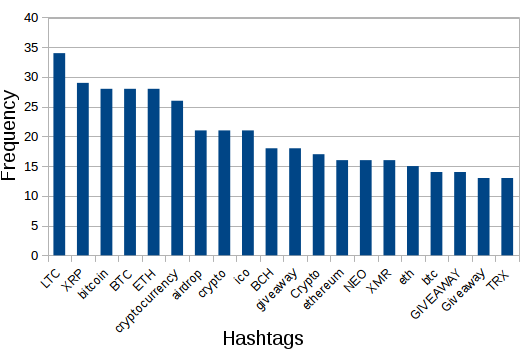
\includegraphics[width=0.4\textwidth]{hashtags_hist}
\caption{Top 20 most used hashtags}
\label{fig:hashtags}
\end{figure}